\section{\label{sec:verification}Verification}
Although the model contains the relevant SEOP physics, it is necessary to verify that the model is providing an adequate computational solution to those expressions. In order to confirm that the FEM model conformed to accepted results, a comparison study was run with the model described by in Ref. \cite{Freeman2014}. 

The model described by Ref. \cite{Freeman2014} differs from the model described here is several important ways. The numerical method used by Ref. \cite{Freeman2014} model is finite-difference method rather than a finite element method. The Ref. \cite{Freeman2014} model is a one-dimensional simulation. The fluid velocity, temperature, and the Rb density distribution are approximated as uniform in the Ref. \cite{Freeman2014} model. The laser spectral profile used in the Ref. \cite{Freeman2014} model is not constrained to be Gaussian; rather spectral profile is discretized and calculated at each spacial node in the model. Finally, the $^{129}$Xe polarization is calculated using the average Rb polarization rather than Rb polarization at each spacial node.

It was possible to reproduce aspects of this model in the infrastructure of FEM model described here. The geometry of the FEM model was drawn as a cylinder. The Navier-Stokes fluid model, heat transfer mode, and Rb diffusion model were disabled. They were replaced with uniform axial flow, a uniform temperature, and a homogeneous Rb number density. The outlet xenon polarization of this FEM model was compared with the predicted xenon polarization from the Ref. \cite{Freeman2014} model.  

The results of this comparison are shown in Figure \ref{fig:modelcomparison}. The two models predicted very close to the same polarization at low temperature for all flow velocities. The discrepancy between the models increases with both the temperature and the flow velocity. The Ref. \cite{Freeman2014} model nearly always predicts a lower polarization. The largest absolute and relative discrepancies are 9 percentage points (16\%) and 19\% (8 percentage points), respectively.

\begin{figure}
    \centering
    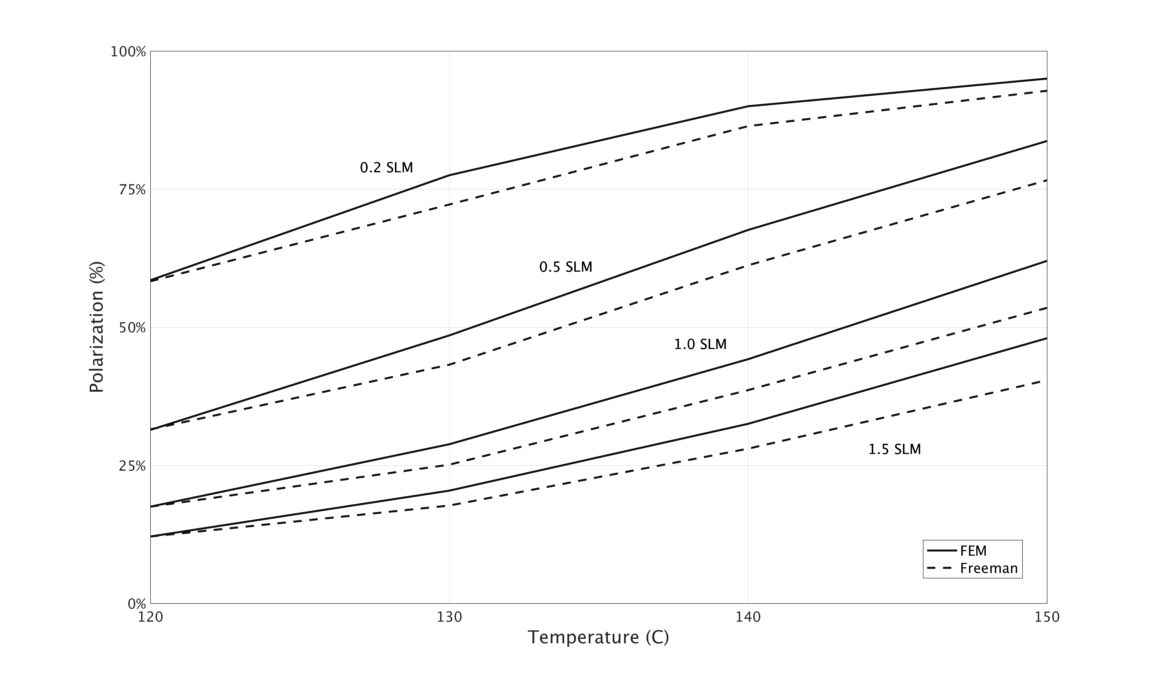
\includegraphics[width=0.5\textwidth]{Figures/FEM_vs_Freeman.png}
    \caption{The predicted $^{129}$Xe polarization from the Ref. \cite{Freeman2014} model and the current model (FEM) as a function of temperature and flow velocity. Each curve represents a different flow velocity (0.2, 0.5, 1.0, and 1.5 SLM) from a different model. The dotted lines are the predictions of Ref. \cite{Freeman2014}, and the solid lines are the predictions of the FEM model. The Ref. \cite{Freeman2014} model almost always predicts a lower polarization than the FEM model. This is thought to be due to a combination of the FEM model including diffusion in the $^{129}$Xe polarization solver and the FEM model using a heterogeneous Rb polarization.}
    \label{fig:modelcomparison}
\end{figure}

A couple explanations for this discrepancy were considered and rejected. One explanations for this discrepancy is that the calculated laser absorption differs in the two models. The Ref. \cite{Freeman2014} model does not enforce the assumption of a Gaussian spectral profile of the laser, while the FEM model described here does. The assumption of a Gaussian spectral profile might influence the calculated Rb polarization, and thus the final $^{129}$Xe polarization. However, when a comparison of the 0.2 SLM flow-rate series was conducted, it was both found that the average calculated Rb polarization differed by no more than 0.2 percentage points (0.2\%) and that the Ref. \cite{Freeman2014} model usually predicted a \textit{higher} Rb polarization. 

Another possible cause was the Rb polarization gradient in the FEM model created the discrepancy between the two models. Although the Ref. \cite{Freeman2014} model does calculate a spacial gradient in the Rb polarization, the final $^{129}$Xe polarization calculation uses a spatially-averaged value. In order to test if this was the cause of the discrepancy, the  flow direction in the FEM model was reversed so that it was directed parallel to the direction of laser propagation instead of anti-parallel. Although this did result in a  lower prediction of the $^{129}$Xe polarization, the affect was not sufficient to account for the discrepancy between the Ref. \cite{Freeman2014} model and the FEM model. 

A final possibility is that FEM model incorporates diffusion while the Ref. \cite{Freeman2014} model does not. This difference, coupled with a Rb polarization gradient, will cause the FEM model to predict higher $^{129}$Xe polarizations than the Ref. \cite{Freeman2014} model by significant amounts. The solution to the one-dimensional diffusion-reaction equation, assuming a linear Rb polarization as a function of axial position, causes the final predicted $^{129}$Xe polarization to fall off linearly as a function of gas velocity. Solving the advection-reaction equation (used in the Ref. \cite{Freeman2014} model) with a Rb polarization independent of axial position causes the final predicted $^{129}$Xe polarization to fall off exponentially with gas velocity. This is likely the cause of the discrepancy between the predictions of the two models. 